%-------------------------------------------------------------------------------
%                            BAB I
%                          PENDAHULUAN
%-------------------------------------------------------------------------------

\chapter{PENDAHULUAN}

\section{Latar Belakang}
\blindtext

Penelitian ini didasarkan pada persamaan fundamental fisika kuantum yang menggambarkan tingkat energi atom hidrogen:

\begin{equation}
E_n = -\frac{13.6 \text{ eV}}{n^2}
\label{eq:energy-levels}
\end{equation}

di mana $n$ adalah bilangan kuantum utama dan $E_n$ adalah energi tingkat ke-$n$.

\blindtext

\section{Rumusan Masalah}
\blindtext

Permasalahan utama dapat diilustrasikan pada Gambar \ref{fig:diagram-masalah} berikut:

\begin{figure}[htbp]
\centering
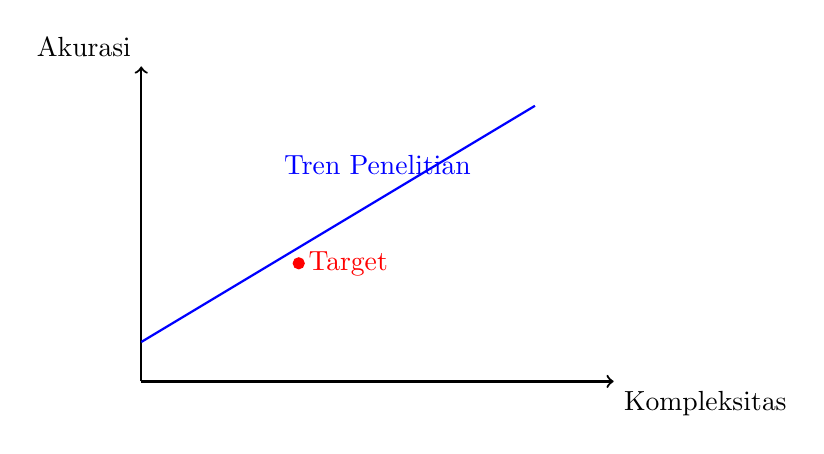
\begin{tikzpicture}
\draw[thick,->] (0,0) -- (6,0) node[anchor=north west] {Kompleksitas};
\draw[thick,->] (0,0) -- (0,4) node[anchor=south east] {Akurasi};
\draw[blue,thick] (0,0.5) -- (5,3.5);
\node at (3,2.5) [above,blue] {Tren Penelitian};
\filldraw[red] (2,1.5) circle (2pt) node[anchor=west] {Target};
\end{tikzpicture}
\caption{Diagram permasalahan penelitian}
\label{fig:diagram-masalah}
\end{figure}

\section{Tujuan Penelitian}
\blindtext

\section{Batasan Penelitian}
\blindtext

\section{Manfaat Penelitian}
\blindtext
